\documentclass[a4paper,12pt]{article}

\usepackage[T1]{fontenc}
\usepackage[utf8]{inputenc}
\usepackage{lmodern}
\usepackage[top=2cm, bottom=3cm, left=1.5cm, right=1.5cm]{geometry}
\usepackage{fancyhdr}
\usepackage[pdftex]{graphicx}
\usepackage{graphics}
\usepackage{float}
\usepackage{latexsym}
\usepackage{amsmath,amsfonts,amssymb}
%\usepackage{tikz}
% \usepackage{placeins}
% \usepackage[french, figure, boxed, longend]{algorithm2e}
\usepackage[francais,english]{babel}


% % En-t�tes et pieds de page
% \pagestyle{fancy}
% \headheight 35pt
% \lhead{\textbf{\begin{small}Rapport Projet 2008-2009\end{small}}}
% \chead{\textsc{\begin{large}Etude de la topologie de l'Internet\end{large}}}
% \rhead{\textbf{\begin{small}\end{small}}}
% \lfoot{2008}
% \rfoot{\thepage}
% \cfoot{}

\pagestyle{fancy}
\renewcommand{\sectionmark}[1]{\markright{\thesection\ #1}}
\renewcommand{\headrulewidth}{0.5pt}
\renewcommand{\footrulewidth}{0.5pt}
\fancyhead{} % clear all header fields
\fancyhead[L]{Etude de la topologie de l'Internet}
\fancyhead[R]{\rightmark}
\fancyfoot{} % clear all footer fields
\fancyfoot[C]{\thepage}


\newcommand{\boost}{\textit{Boost }}
\newcommand{\Hrule}{\rule{\linewidth}{0.5mm}}

%opening
\title{Etude du coeur de l'Internet}
\author{Jan Villeminot \& Bastien Legrand}

\begin{document}
\selectlanguage{francais}
%\begin{changemargin}
\begin{titlepage}
	\begin{minipage}{0.5\textwidth}
		\begin{flushleft} \large
			%
\includegraphics[bb=0 0 110 30]{images/logo-isima.png}\\
			
\includegraphics[width=3.8cm]{./schema/logo-isima.jpg}\\
		\end{flushleft}
	\end{minipage}
	\begin{minipage}{0.43\textwidth}
		\begin{flushright} \large
			
\includegraphics[width=3.8cm]{schema/logo-boost.png}
		\end{flushright}
	\end{minipage}

	\begin{minipage}{0.5\textwidth}
		\begin{flushleft} \large
			\textbf{I}nstitut \textbf{S}upérieur\\
			d'\textbf{I}nformatique de\\
			\textbf{M}odélisation et de\\
			leurs \textbf{A}pplications\\
			~\\
% 			\begin{small}
% 			Complexe des Cézeaux \\
% 			BP 125\\
% 			63173 Aubière Cedex
% 			\end{small}
		\end{flushleft}
	\end{minipage}
	\begin{minipage}{0.43\textwidth}
		\begin{flushright} \large
		\end{flushright}
	\end{minipage}


		\vfill
		\begin{center}
			\Hrule \\[0.4cm]
			\Large{Rapport de Projet de troisième année}\\		
			\Large Filière 5 : Infrastructure entreprise, réseaux et télécoms\\[1.0cm]
			\Huge{Représentation et analyse de la topologie internet}\\
			\Hrule\\[0.8cm]
\vfill 
% \textcolor{red}{\Huge{\textbf{MERCI JULIEN !}}}
% \vfill 
		\end{center}
		
		\vfill
		\begin{minipage}{0.5\textwidth}
			\begin{flushleft} \large
				\emph{Auteurs:}\\
				 Bastien \textsc{Legrand}\\
				 Jan \textsc{Villeminot}

			\end{flushleft}
		\end{minipage}
		\begin{minipage}{0.45\textwidth}
			\begin{flushright} \large
				\emph{Tuteur de projet:} \\
				Mickael \textsc{Meulle}\\
			\end{flushright}
		\end{minipage}
		
		\vfil
		\begin{center}
			{\large 2008-2009}
		\end{center}
	\end{titlepage}
%\end{changemargin}

\newpage
\thispagestyle{empty}
\tableofcontents

\newpage
\thispagestyle{empty}
\listoffigures


\newpage

\addtocontents{toc}{\protect\contentsline{section}{R\'esum\'e}{}}
\begin{abstract}
%\par
Internet, le réseau des réseaux, est une interconnexion de systèmes autonomes, réseaux indépendents et raccordés entre eux. Compte tenu de sa taille, représenter Internet est une entreprise des plus difficiles.

Le projet avait pour but de réaliser un outil permettant d'afficher et d'analyser la topologie de l'Internet. La finalité est de proposer un programme évolutif qui facilite l'implémentation de nouvelles méthodes d'affichage et d'analyse. Ses objectifs en cachent un plus pédagogique : maîtriser les outils à notre disposition et les utiliser lors du développement du logiciel.

Articulé autour du patron Modèle Vue Contrôleur, le logiciel est basé sur la librairie graphe de \boost qui réalise tous les traitements de construction et de manipulation sur la topologie. L'interface graphique, réalisée en Qt est totalement indépendante de la partie traitement et permettra donc l'ajout de fonctionnalités facilement.

En cons\'equence, le travail de d\'eveloppement est parallelisable : une personne travaillant plus sur l'interface graphique, l'autre sur la couche de coeur. L'association des diff\'erentes parties est facilit\'ee par l'utilisation d'un gestionnaire de source : git.

L'affichage de la topologie a un rendu circulaire et est accompagné d'une fonction de zoom et d'un certain nombre de fonctions de filtrage et de calcul pour permettre à l'utilisateur, selon ses besoins, de se focaliser sur un aspect précis du graphe.

Finalement, l'outil r\'ealis\'e est \'evolutif, performant et son d\'eveloppement nous a permis d'approfondir nos connaissances dans les outils utilis\'es.\\

mots cl\'e : boost, Qt, interface graphique, évolutivité, topologie de l'Internet, git








\end{abstract}
\thispagestyle{empty}


\newpage
\selectlanguage{english}
\addtocontents{toc}{\protect\contentsline{section}{Abstract}{}}
\begin{abstract}

\end{abstract}
\thispagestyle{empty}


\selectlanguage{francais}
\newpage
\fancyhead[R]{Lexique}
% \documentclass[a4paper,10pt]{article}

% \begin{document}

\section*{Lexique}

\subsection*{clique / full-mesh}

Ensemble de sommets deux \`a deux adjacents.

\subsection*{Syst\`eme Autonome AS}

Un Syst\`eme Autonome est un ensemble de r\'eseaux IP sous le contrôle d'une seule et m\^eme entit\'e administrative, et ob\'eissant \`a une politique de routage interne coh\'erente.

\subsection*{graphe connexe}

En th\'eorie des graphes, un graphe est connexe s'il existe un chemin reliant chaque couple de sommet du graphe.

\subsection*{centralit\'e}

En th\'eorie des graphes, la centralit\'e est une mesure de l'importance d'un arc ou d'un sommet dans le graphe.

% \end{document}



\newpage
\fancyhead[R]{\rightmark}
\section{Visualisation de la topologie inter-domaine de l'Internet}

% \documentclass[a4paper,10pt]{article}

% \begin{document}

\subsection{Tomographie de l'Internet inter-domaine}

\subsubsection{Pr\'esentation d'Internet}

\par
Aujourd'hui, le r\'eseau le plus connu de part le monde est l'Internet. Il est le fruit combin\'e de la recherche militaire et de l'inter\^et que lui ont ensuite port\'e les universitaires.
\par
%TODO Déplacer en Accroche d'introduction doit pas être là ce truc... mais gg pala ça a la classe pour l'accroche.
Au d\'ebut utilis\'e pour relier entre eux les principaux sites militaires des \'Etats-Unis, puis les universit\'es, Internet relie aujourd'hui des millions de foyers de part le monde, mais que se cache-t-il r\'eellement derri\`ere cette appellation?
\par
%TODO Fin deplacer
Internet est en fait un r\'eseau de r\'eseaux. Des r\'eseaux ind\'ependants appartenant \`a des entreprises priv\'ees, des universit\'es, des op\'erateurs. Ces r\'eseaux ind\'ependants sont appel\'es syst\`emes autonomes AS. Chaque r\'eseau est connect\'e \`a plusieurs autres et lorsque deux ordinateurs appartenant \`a des AS diff\'erents souhaitent communiquer, leurs paquets de donn\'ees seront rout\'es \`a travers l'Internet en passant par plusieurs AS interm\'ediaires. Aucun des \'el\'ements ne connait la totalit\'e de la topologie du r\'eseau et les paquets sont dirig\'es suivant des r\`egles de routage locales.
\par
Lorsque l'on parle de repr\'esenter Internet sous forme de graphe, dans la pr\'esente \'etude, il s'agit en fait de repr\'esenter les liens entre les diff\'erents AS. Cependant, il est n\'ecessaire de connaitre la topologie inter-AS au pr\'ealable pour pouvoir la repr\'esenter.

\subsubsection{Origine des donn\'ees}
\par
Il existe diff\'erents outils pour connaitre les liens entre les diff\'erents AS. Comme indiqu\'e sur le site \textit{www.caida.org} il existe au moins trois outils pour obtenir la topologie inter-AS :
\begin{description}
 \item[traceroute : ] outil permettant de capturer les adresses IP des diff\'erents \'equipements r\'eseau sur un chemin entre une source et une destination en utilisant des paquets sonde UDP ou ICMP. La r\'esolution du num\'ero d'AS associ\'e \'a chaque adresse IP permet d'obtenir une carte inter-AS.
 \item[BGP : ] protocole de routage inter-domaine utilis\'e pour le routage entre les AS. Ses tables de routage contiennent des chemins d'AS, on peut ainsi avoir une idée des liens entre les diff\'erents AS.
 \item[WHOIS : ] collection de bases de donn\'ees contenant des informations utiles aux op\'erateurs. Malheureusement, ces bases de donn\'ees sont maintenues \`a la main et ne  sont donc pas toujours tr\`es fiables. La plus sûre est la RIPE WHOIS qui regroupe des informations collect\'ees par la RIPE (service d'information sur les R\'eseaux IP Europ\'eens).
\end{description}
\par
Nous utiliserons principalement la m\'ethode BGP en raison de sa fiabilit\'e.

\subsubsection{Internet IPv4 et IPv6}
\par
Aujourd'hui, un changement majeur qui est en train de s'op\'erer dans les r\'eseaux : le passage de l'IPv4 \`a l'IPv6. En effet, si IPv4 permet l'utilisation d'un peu plus de quatre milliards d'adresses ($2^{32}$), IPv6 permet quant \`a lui d'utiliser $2^{128}$ adresses diff\'erentes, ce qui permet de combler les nouveaux besoins.
\par
La mise en place progressive de l'IPv6 se traduit au sein des grands r\'eseaux par une cohabitation entre les deux syst\`emes. On peut ainsi trouver des informations pour cr\'eer le graphe de topologie pour l'internet IPv4 mais aussi pour l'internet IPv6.
\par
Au cours de notre projet, nous avons eu successivement acc\`es aux donn\'ees de l'IPv4 puis de l'IPv6.
% \end{document}


%\documentclass[a4paper,12pt]{article}

%\usepackage{graphics}
%\usepackage[pdftex]{graphicx}

%\begin{document}

\subsection{Topologie de l'Internet}
\par
Commme expliqu\'e pr\'ec\'edemment Internet n'est pas un seul est grand r\'eseau, il s'agit en fait de l'interconnection de plusieurs r\'eseaux ou syst\`emes autonomes (AS). Un syst\`eme autonome est un r\'eseau r\'egit par une administration et soumis \`a un ensemble de r\`egles de routage internes. Les AS sont reli\'es entre eux par diff\'erents types de liens. Ces liens peuvent \^etre :
\begin{description}
 \item[PEER] il s'agit d'un accord commercial \`a travers lequel les clients respectifs de deux AS peuvent communiquer entre eux sans que les AS ne doivent se payer la connection,
 \item[P2C ou C2P] il s'agit d'un lien commercial \`a travers lequel un AS devient le client d'un autre et peut faire transf\'erer son trafique r\'eseau.
\end{description}
\par
Au coeur de l'Internet, on trouve les op\'erateurs appel\'es \textit{Tier One} qui sont reli\'es deux \`a deux par des liens de type PEER. Il s'agit l\`a d'une structure type full-mesh aussi appel\'ee \textit{clique} en th\'eorie des graphes.
\par
On trouve reli\'es \`a ces grands op\'erateurs d'autres AS qui peuvent eux-m\^eme \^etre reli\'es \`a d'autre et ainsi de suite. De fa\c con locale, on peut retrouver des full-mesh.
\par
Globalement, Internet a une structure connexe, c'est-\`a-dire que si l'on prend deux AS au hasard, il existe un chemin qui les relie.
\par
Il revient \`a chaque AS d'assurer la visibilit\'e de ses clients \`a travers le r\'eseau.
\par
En bout de cha\^ine, il y a des feuilles. Ce sont des AS qui sont clients d'un ou plusieurs autres AS mais qui n'ont pas de client \`a eux. Quand un AS feuille est reli\'e \`a un seul AS, on dit qu'il est \textit{monohom\'e}, si au contraire, il est le client de plusieurs autres AS en m\^eme temps, on dit alors qu'il est \textit{multi-hom\'e}.


\subsubsection{Repr\'esentation d'Internet}
\par
De fa\c con pratique, on peut repr\'esenter Internet comme un graphe o\`u les sommets sont les AS et les ar\^etes les liens entre les AS. La figure suivante montre un exemple de cette repr\'esentation avec un coeur de l'Internet compos\'e de trois AS auxquels sont connect\'es d'autres AS. On remarque que certain AS peuvent \^etre client aupr\`es de plusieurs AS en m\^eme temps. Cette m\'ethode est utile pour garantir un connectivit\'e m\^eme en cas de d\'efaillance d'une connection.

\begin{figure}[ht]
\centering
 \fbox
 {
 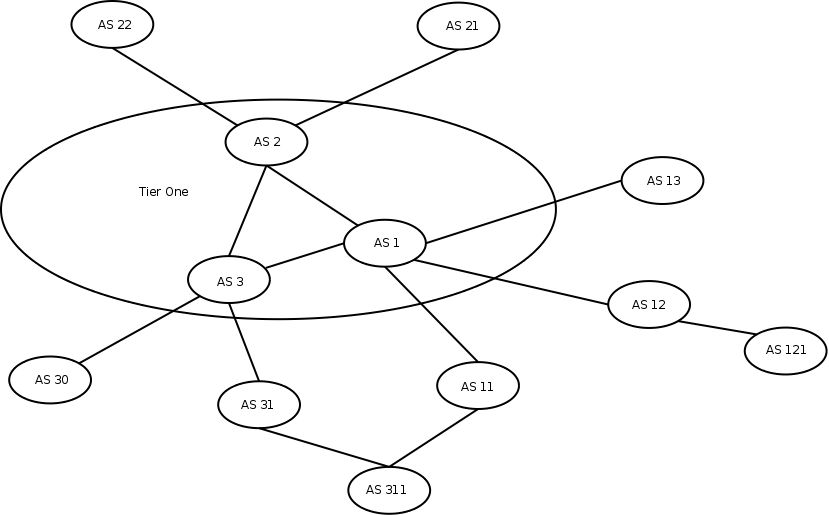
\includegraphics[width=16cm]{./schema/topologie_internet.png}
 }
  \caption{\label{topologie}Topologie d'Internet, exemple de repr\'esentation}
\end{figure}



%\end{document}


%\documentclass[a4paper,12pt]{article}


%\begin{document}

\subsection{Analyse de la topologie}

\par
Pour analyser la topologie de l'Internet \`a partir du graphe le repr\'esentant, nous disposons de plusieurs outils fournis par la th\'eorie des graphes.

\subsubsection{Les cliques}

Tout d'abord, la recherche des cliques permet d'identifier les endroits o\`u les AS sont tous reli\'es deux \`a deux, un de ces ensembles est constitu\'e des op\'erateurs du \textit{Tier One}. On retrouve aussi d'autres cliques localement.
%TODO peut etre a compléter

\subsubsection{La centralit\'e}

\par
Ensuite, comme il a été expliqu\'e lors de la pr\'esentation de la topologie de l'Internet, le graphe a une structure connexe, c'est-\`a-dire que si l'on prend deux sommets quelconques, il existe un chemin entre ces deux sommets.
Ce chemin passe par un certain nombre d'ar\^etes, et il est int\'eressant de savoir si telle ou telle ar\^ete est plus importante.
\par
Prenons l'exemple de deux AS A et B reli\'es entre eux. Nous savons qu'il existe une ar\^ete sur notre graphe entre A et B, supposons alors qu'il n'existe pas d'autres liens que celui entre A et B pour que les clients de A puissent joindre les clients de B. Ce lien revet donc une importance capitale puisque l'ensemble des routes partant des clients de A vers les clients de B passent par celui-ci.
\par
Il nous faut alors assigner des poids aux liens ou aux sommets afin de tenir compte de leur importance dans la structure globale.

\par
En th\'eorie des graphes, il existe un outil permettant d'\'evaluer l'importance des sommets ou des ar\^etes d'un graphe : la \textit{centralit\'e}. La centralit\'e permet de calculer le ratio du nombre de chemins passant par cette ar\^ete ou ce sommet par rapport au nombre de chemins total dans le graphe. Plus ce ratio est important plus le noeud ou l'ar\^ete est vital pour garder le caract\`ere connexe du graphe. La centralit\'e se calcule gr\^ace \`a la formule suivante :

\begin{figure}[!ht]
   \centering
   \frame
   {
      \parbox{12cm}
      {
         Soit un graphe G=(V,E) avec n sommets, la centralité $c_b(v)$ d'une arête v est :
         \begin{equation}
               c_b(v) = \sum_{\underset{s \neq v}s \neq v \neq t V} \frac{\sigma_st(v)}{\sigma_st}
         \end{equation}
	o\`u $\sigma_st$ est le nombre de plus court chemin allant de s vers t et $\sigma_st(v)$ est le nombre de plus court chemin de s vers t passant par v.
      }
   }
  \caption{\label{centralit\'e}Calcul de la centralit\'e}
\end{figure}



%\end{document}


% \documentclass[a4paper,10pt]{article}

% \begin{document}

\subsection{Repr\'esentation de la topologie}

Repr\'esenter Internet sous la forme d'un graphe peut s'av\'erer particulièrement difficile. En effet, si l'on regarde les donn\'ees r\'ecolt\'ees au niveau de diff\'erentes sources, on s'aperçoit que le graphe \`a repr\'esenter est immense : pour la topologie IPv4, il comporte plus de 40000 sommets et un nombre tout aussi cons\'equent d'ar\`etes.
\par
La topologie en IPv6 est \`a peine plus petite. Cela vient du fait que cette technologie n'est pas encore aussi largement r\'epandue que l'IPv4.

\par
Au tout d\'ebut du projet, nous avons essayé de repr\'esenter le graphe complet, avec tous ses sommets et toutes ses ar\^etes. Le r\'esultat obtenu \'est, comme on peut s'y attendre, confu et illisible. Il nous a donc fallu envisager des solutions pour all\'eger nos traitements et notre affichage.
\par
Voici une capture d\'ecran du programme lorsqu'il repr\'esente le graphe dans son int\'egralit\'e :
%TODO insérer ici une capture d'écran avbec le graphe complet
%TODO faire une figure et la référencer dans le paragraphe
\par
Le principe est de nettoyer le graphe en enlevant les AS feuilles qui sont tr\`es nombreux et pas nécessairement tr\`es pertinents pour une \'etude de la topologie du coeur de l'Internet. 
\par
%TODO Deplacer en partie IV, c'est l'élaboration du logiciel, contrairement à la partie 1 qui traite d'autre chose...
Dans un premier temps, on cible les AS qui n'ont ni client, ni PEER. Ce sont n\'ecessairement des feuilles, et par cons\'equent, nous pouvons les retirer du graphe pour faciliter sa lecture et alléger nos calculs.
\par Ensuite, notre tuteur de projet, Monsieur Meulle, nous a donn\'e un nouveau fichier, avec des relations entre AS sous la forme de triplets, permettant d'identifier tr\`es rapidement les AS feuilles.
Les liens entre AS sont plac\'ees sous la forme de triplets : {AS1, AS2, AS3} signifiant que ppour joindre l'AS3, l'AS1 a du passer par l'AS2. Ainsi, on peut identifier les AS de transit (ici l'AS2). Les AS feuilles sont alors facilement identifiables comme \'etant ceux qui ne jouent jamais le r\^ole d'As de transit dans les triplets.
%TODO Fin du déplacer...
\par
\'Etant donn\'e qu'Internet joue aujourd'hui un r\^ole important dans notre vie de tous les jours, tant au niveau professionnel que priv\'e, plusieurs \'etudes ont d\'ej\`a \'et\'e men\'ees pour mieux en comprendre la structure.
On trouve ainsi plusieurs ouvrage dans la litt\'erature et sur le net qui parle de ce sujet. On peut aussi trouver divers repr\'esentation graphique de l'Internet.
%TODO on pourrait ajouter cette image avec un commentaire, elle est sympa : http://en.wikipedia.org/wiki/File:Internet_map_1024.jpg

%\end{document}

\pagebreak
\section{Le logiciel de visualisation et d'analyse de l'internet}
\subsection{Objectifs}
Le but du projet est de produire un logiciel qui permette la visualisation de la topologie d'internet :
\subsubsection{Objectifs de l'application}
\label{obj}
\paragraph{Analyse de la topologie}
Construire un graphe contenant la topologie d'internet et permettant son analyse en se servant des méthodes disponibles dans la librairie graphe de \textit{Boost}.

\paragraph{Affichage de la topologie}
Réaliser une interface agréable dans la librairie de notre choix et lui permettre d'afficher l'intégralité de l'analyse réalisée.

\subsubsection{Objectif pédagogiques}
Au delà, de l'objectif de réalisation d'une application et de l'organisation que cela suppose. Un certains nombre d'objectifs pédagogique ont été fixés par notre tuteur ou par nous-même.

\paragraph{Objectifs fixés dès le départ : } 
\paragraph{}L'objectif principal est bien évidemment d'apprendre à maîtriser la librairie boost de C++, principalement sa partie sur les graphs. Il était aussi question d'approfondir notre connaissance de la topologie d'internet.

\paragraph{Objectifs personnels suppl\'ementaires : }
\paragraph{} En outre, nous nous sommes nous-même fixés des objectifs. En effet, l'utilisation d'une librairie graphique pour représenter la topologie d'internet était nécessaire mais son choix nous était réservé. Nous avons choisi d'utiliser Qt, et ce pour deux raisons. La première est que nous voulions approfondir le cours sur Qt que nous allions avoir dans le cadre de nos études à l'ISIMA.

La seconde est que, sous la pression de Nokia, cette librairie est récemment passé sous licence LGPL ce qui veut dire que les développeurs d'applications commerciales vont pouvoir développer gratuitement autour de Qt (sans payer les très onéreuses licences jusqu'à présent nécessaires pour vendre quelque chose). Il est fort probable que Qt prennent beaucoup plus d'ampleur dans les prochaines années.

\paragraph{} Nous nous sommes fixés un autre objectif, celui d'apprendre à utiliser git, pour les raisons évoqué en \ref{gitPar} subversion ne nous convenait pas, mais nous ne connaissions pas vraiment git pour autant, néanmoins après avoir visionner une conférence de Linus Torvalds sur le sujet, il nous a semblé logique et nécessaire d'appréhender git et de s'en servir pour le projet. D'autant plus que l'un comme l'autre nous avions effectué nos stages avec subversion ou cvs.

\subsubsection{Déroulement du projet}

Nous n'avons que très peu vu notre tuteur de projet en personne, la quasi totalité du projet a été mené par des échanges de mails, et des discussions sur des messageries instantannées (Skype, gchat). De plus, il nous a donné une grande autonomie sur les décisions à prendre pour mener à bien nos objectifs.

En contre-partie, cela demande une bonne organisation. En effet, quelques soient les décisions ou les problèmes rencontrés, il faut en rendre compte au tuteur lors de la prochaine réunion de travail suivante, réunion qui avait régulièrement lieu le Jeudi après-midi.

\subsubsection{Méthode de travail}

Afin d'optimiser la production, nous avons adopté une méthode de développement par itération. En fait, nous nous sommes répartis les tâches selon des fonctionnalités ``élémentaires'', par exemple afficher le graph avec Circle Graph Layout ou réaliser l'extension du file\_parser permettant de trouver les AS de transit. Après avoir isolé l'ensemble des fonctionnalités nécessaires d'une semaine à l'autre, nous affectons des priorités aux une est aux autres afin de pouvoir mieux répartir les tâches entre les différents membres du binôme.

\subsubsection{La librairie graph de boost}
%\documentclass[a4paper,12pt]{article}

%\begin{document}

% \subsection{La librairie \boost}

\subparagraph{}
La librairie \boost  est un ensemble de biblioth\`eques logicielles C++ dont le but est de compléter et de parfaire les fonctionnalités du langage et la librairie stl. La librairie \boost est compos\'ee de nombreux modules parmis lesquels on retrouve des fonctionnalit\'es de bases comme les entr\'ees / sorties ou la gestion des erreurs, mais aussi d'autres plus avanc\'ees comme des fonctions de gestion de graphes, de programmation lin\'eaire, de g\'en\'eration de nombres pseudo-al\'eatoires, de traitement d'images ou de multithreading.
\par
L'\'ecriture de nouveaux \'el\'ements pour la librairie \boost est soumise \`a un  comit\'e de lecture et l'ensemble des biblioth\`eques est plac\'e sous une licence sp\'eciale : la \textit{Boost Software Licence} qui permet d'inclure des modules \boost aussi bien dans des projets Open Source que dans des projets propri\'etaires.
\par
\'Etant donn\'e que nombre des membres du comit\'e de lecture font aussi partie du comit\'e du standard C++, plusieurs biblioth\`eques issues de la \boost ont \'et\'e s\'electionn\'ees pour faire partie de la prochaine norme du C++.
\par
Au cours de notre projet nous avons beaucoup utilis\'e la partie gestion de graphes de \boost ainsi que certaines des fonctions d'entr\'es / sorties am\'elior\'ees.
%\end{document}



\subsubsection{La librairie graphique Qt}
\subparagraph{}
Qt, prononcer ``cute'' de l'anglais joli, est une biblioth\`eque logicielle orient\'ee objet et d\'evelopp\'ee en C++ par la soci\'et\'e \textit{Qt Software}, anciennement connue sous le nom de \textit{Trolltech}. Elle offre des composants graphique permettant entre autre l'acc\`es aux donn\'ees, les connexions r\'eseaux, la gestion des files d'ex\'ecution. Cette biblioth\`eque est aujourd'hui dans sa version quatre.
\subparagraph{}
Qt permet la portabilit\'e des applications par simple recompilation du code source. Elle est support\'ee sous des environnements tels que Unix/Linux, Windows et Mac OS X.
\subparagraph{}
Qt est principalement connue pour \^etre la biblioth\`eque sur laquelle repose l'environnement graphique KDE, l'un des environnements de bureau le plus utilis\'e dans le monde Linux. En outre, un certain nombre d'applications tr\`es connues du grand public utilisent Qt : VLC Media Player, Skype, Google Earth...

\par
L'outil Qt repose sur trois parties essentielles : 
\begin{itemize}
	\item Les slots et les signaux,
	\item Qt Designer,
	\item Le compilateur de meta-objet MOC.
\end{itemize}

\subparagraph{}
Qt Designer est un outil graphique permettant de créer facilement des interfaces graphiques avec Qt, d'y ajouter des panneaux, des boutons et d'y connecter des fonctions sous la forme de signaux et de slots. Au cours de notre projet, nous n'avons que tr\`es peu utilis\'e cet outil, pr\'ef\'erant explorer les \'etapes de cr\'eation d'une interface graphique en r\'ealisant nous m\^eme tout le code.
\subparagraph{}
Les slots et signaux sont les m\'ecanismes sp\'ecifiques \`a Qt qui lui permettent de g\'erer les \'echanges d'informations entre les diff\'erents \'el\'ements d'une interface graphique. Il s'agit en fait d'une impl\'ementation un peu particulière du patron de conception observateur.
Les objets Qt poss\`edent des slots et des signaux. Un objet peut \'emettre des signaux qui seront re\c cus par les slots d'un autre objet. Ainsi, si on veut cr\'eer un bouton ``quitter'' dans une fen\^etre, il faut connecter le signal correspondant à l'action \textit{je clique sur le bouton} au slot \textit{la fen\^etre se ferme}.
\subparagraph{}
Le compilateur de m\'eta-objets MOC (Meta Object Compiler) est un pr\'eprocesseur qui est appliqu\'e au code source de l'application avant sa compilation et qui r\'eunit les informations n\'ecessaires au fonctionnement des slots et signaux, voir \'eventuellement \`a l'introspection. \subparagraph{}
L'introspection est la capacit\'e qu'a un programme à connaître son \'etat, examiner ses structures internes et \'eventuellement modifier des objets le composant au cours de l'\'execution. Cela va de pair avec les slots et les signaux, puisque pour cacher une fen\^etre, on peut ainsi changer son \'etat de visible \`a non visible.
Un exemple d'introspection est le démon dcop de KDE qui permet de connaitre exactement l'état de chaque composant d'une application KDE, et d'agir dessus. Il est par exemple possible d'arrêter la musique avec Amarok, ou de graver un CD uniquement par introspection avec K3B.
Non présente nativement en C++, la faisabilité de l'introspection est un atout majeur de Qt.

\subsection{Méthodologie de développement et redistribution}
\subsubsection{Documentation avec Doxygen}
\par
Doxygen est un outil permettant la génération de documentation à propos de code, il est utilisable avec la plupart des langages de programmation actuels (C/C++, Java, python, Groovy). Son nom est la contraction de \textit{dox} (pour docs, de l'anglais documents) et \textit{gen} (de l'anglais generator). Il a été en grande partie \'ecrit par Dimitri van Heesch. La documentation g\'en\'er\'ee peut \^etre soit en HTML, soit en \LaTeX.

\par Il s'appuie pour cela sur un certains nombre de commentaires \'ecrits dans le code avec une syntaxe sp\'ecifique (voir figure \ref{exemple_doxygen}). Il se base aussi sur une analyse du code qui lui permet d'extraire les prototypes des fonctions, des classes, les fichiers inclus et la documentation relative à ceux-ci.

\par Il peut ensuite repr\'esenter leur hi\'erarchie sous forme de sch\'emas UML. Il crée ensuite une documentation homogène permettant de naviguer à partir d'un index vers les différentes pages de documentation créées.

	La figure 3 nous montre comment définir une br\`eve description du r\^ole de la méthodes, des informations sur ses diff\'erents param\`etres et sur ce qu'elle retourne.

\begin{figure}[H]
        \begin{center}
                \begin{tabular}{l}
                        \hline
                        \verb|\brief Ajoute une arete|\\
                        \verb|\param i1 index du premier point|\\
                        \verb|\param i2 index du deuxieme point} |\\
                        \verb|\param linkType descripteur du type d'arete|\\
			\verb|\param found booleen resultat |\\
			\verb|\param e edge_descriptor de l'arete|\\
			\verb|\param g reference sur le Graph ou il faut ajouter la relation|\\
			\verb|\return le type de point|\\
                        \hline
                \end{tabular}
        \end{center}
\caption{\label{exemple_doxygen} Exemple de syntaxe Doxygen}
\end{figure}


\subsubsection{Redistribution et travail en équipe}
\paragraph{subversion : des limites}
%TODO supprimer premier paragraphe
%EvOr se défoule
%La plupart des personnes ayant utilisé subversion de manière professionnelle en sont conscientes il est loin d'être agréable à utiliser, sa gestion des branches est désastreuses, et les conflits sont gérés de manière abruptes et souvent inefficaces, pour palier à ses défauts les entreprises mettent en place des politiques de fonctionnement autour du gestionnaire de version drastique avec par exemple interdiction de commiter ce qui ne marche pas. Au delà de ses problèmes de fonctionnement subversion est lent, très lent et nécessite en plus la présenced'un serveur pour pouvoir commiter.
%Fin EvOr se défoule

\paragraph{} L'une des bases du développement est d'utiliser un gestionnaire de sources afin de pouvoir modifier ses fichiers sans se soucier des conséquences. La première chose que nous avons faite, avant même de passer au développement, est de mettre en place un serveur subversion sur l'une de nos machines. Le problème qui s'est très vite posé est le suivant : quelque soit l'endroit où l'autre travaille, s'il n'a pas accès au serveur, il ne peut pas l'utiliser (\verb|commit/checkout|) et doit donc développer sans gestionnaire de sources (figure \ref{svn})... Il nous fallait un moyen de contrôler nos sources de manière distribuée : git.

\begin{figure}[H]
\begin{center}
        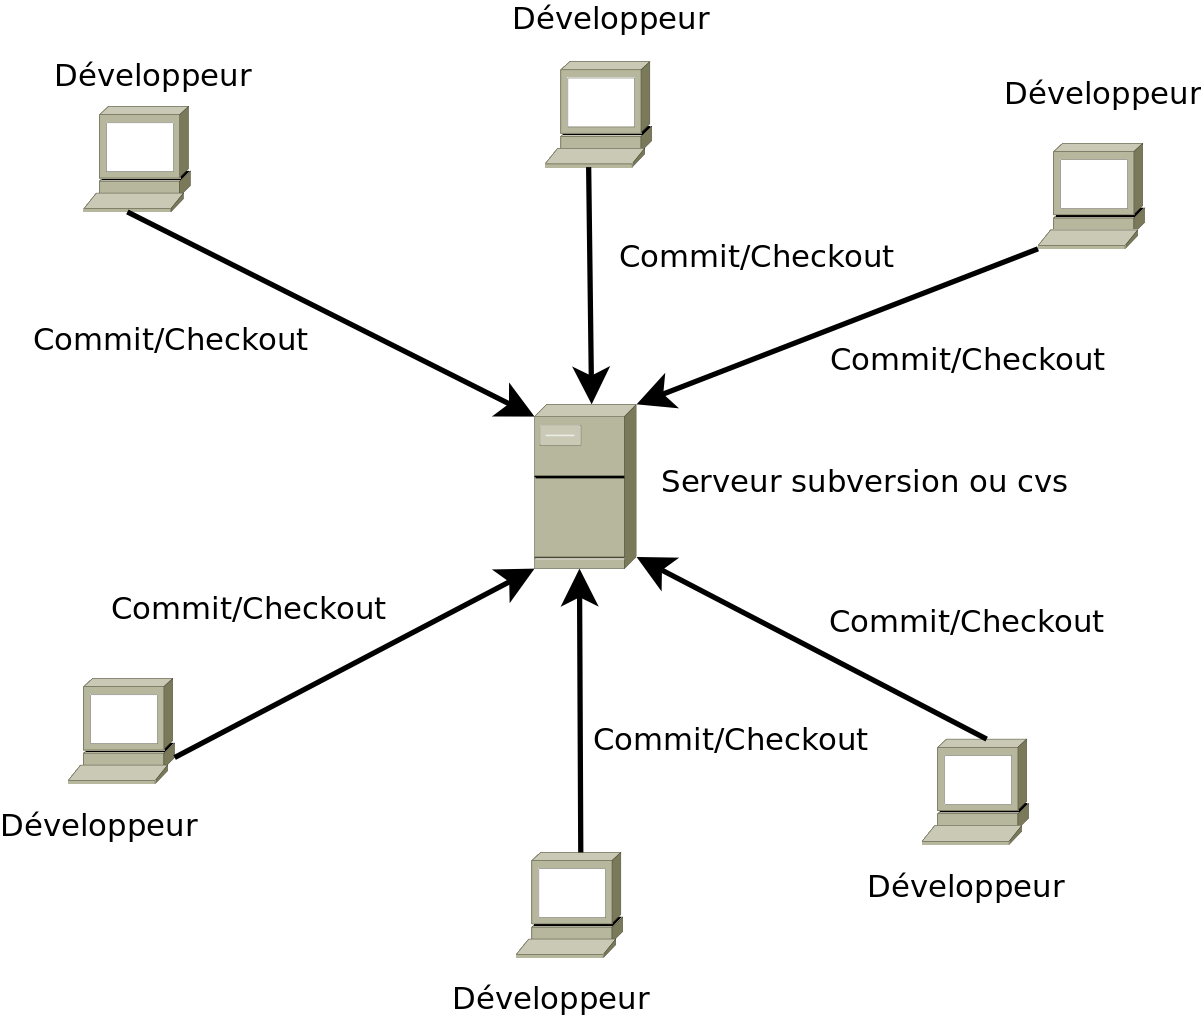
\includegraphics[width=0.7\textwidth]{./schema/svn.png}
\caption{La gestion classique des sources : centralisation totale }
\label{svn}
\end{center}
\end{figure}


\paragraph{git : Le gestionnaire de source distribué}
\label{gitPar}
\paragraph{Histoire :}
\subparagraph{} Git a été créé par Linus Torvalds en 2004, il avait besoin de remplacer BitKeeper pour la gestion des sources du noyau Linux, et il est évident qu'il ne peut pas mettre en place un serveur subversion pour un projet aussi vaste et avec autant de développeurs répartis au quatre coins du monde. Il a donc écrit, en quelques jours, un gestionnaire de sources distribué performant et qui a pour objectif de ne pas géner le développeur. En outre, Git effectue un checksum SHA1 des sources à chaque fois qu'une modifications est effectuée (commit ou push) ce qui permet d'être sûr de l'unicité des données...

\paragraph{Que veut dire distribué ?} 
\subparagraph{}Git est distribué, cela veut dire que chaque machine l'utilisant est un serveur et un client. En d'autres termes, chaque développeur peut ``commiter'' et effectuer des \verb|revert| en local. Ce qui permet de développer de manière beaucoup plus efficace, puisque les commits sont effectués en quelques millisecondes (le temps d'afficher la trace). Une fois que le développeur est satisfait de son travail, il peut demander aux autres de \verb|pull| (récupérer les sources) depuis sa machine, ou il peut \verb|push| (envoyer les sources) sur un serveur de fichiers central par exemple (figure \ref{git}). Tout ce que nécessite git pour fonctionner est un client et/ou un serveur ssh.


\begin{figure}[H]
\begin{center}
        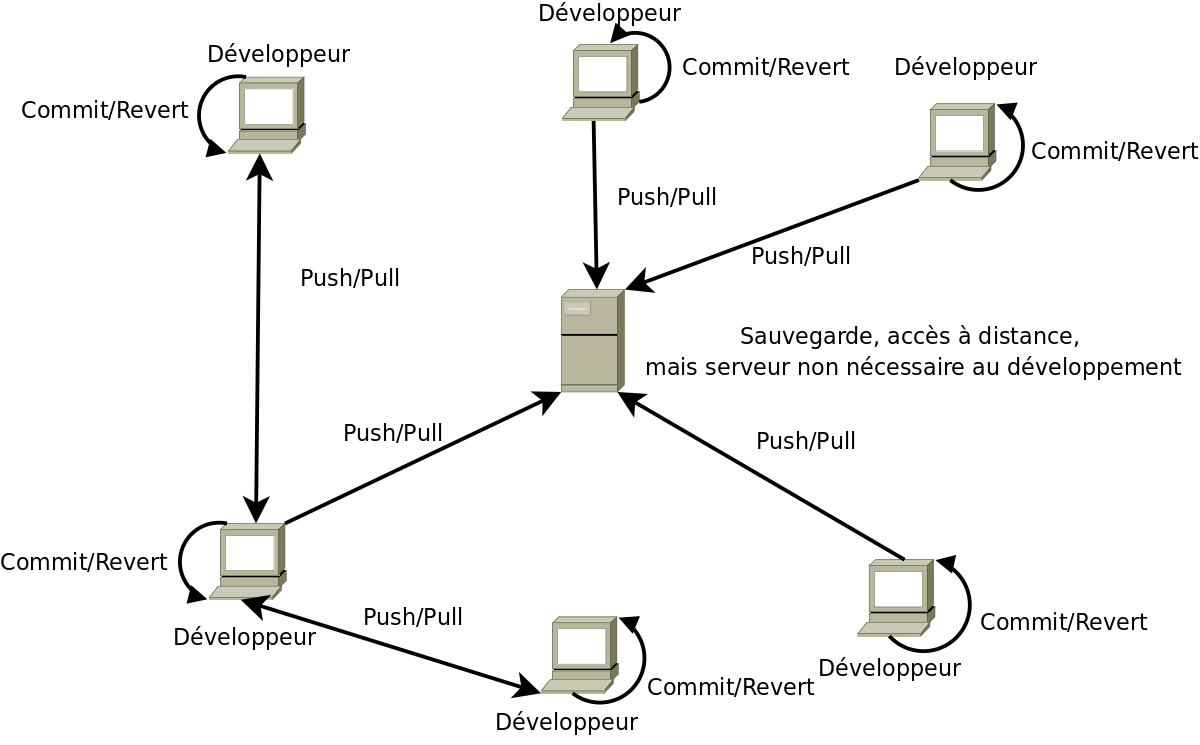
\includegraphics[width=0.8\textwidth]{./schema/git.png}
\caption{La gestion des sources avec git : Distribution et liberté}
\label{git}
\end{center}
\end{figure}

\paragraph{Fonctionnement :} 

\subparagraph{}La comparaison de fichiers sous git est un peu particulière, contrairement à subversion qui se base sur le nom du fichier et le numéro du commit, git se base sur un checksum du fichier. Il se sert en fait d'une base interne contenant l'intégralité des checksums des fichiers en fonction du numéro du commit correspondant mais ne se base que sur le checksum pour vérifier si deux fichiers sont différents, l'opération est donc très rapide et sûr.

\subparagraph{} Concrètement, la clé du fonctionnement de git est l'utilisation massive des branches. En effet, dans git tout est une branche : chaque machine de chaque développeur est une branche et ce de manière totalement transparente. C'est à dire que le développeur peut \verb|commit| et \verb|revert| sa propre branche et l'envoyer ensuite sur la branche principale \verb|push| (\verb|master|). Avec les sources, l'historique des commits effectués en local est envoyé et n'importe quel développeur peut annuler n'importe quel commit...

\subparagraph{} Il est donc très facile de créer, de merger et de supprimer une branche avec git, tellement facile qu'on se demande comment ça peut être aussi difficile avec subversion.

\subparagraph{} En cas de conflit, git ne fait rien ; pour git le simple fait que deux fichiers devant être ``mergés'' soient plus ``récents'' que leur dernière version commune est un conflit. Il signale alors à l'utilisateur qu'il faut ``merger''. Et ce merge est très aisé, il se déroule automatiquement la plupart du temps, à la main parfois : git est capable de ne montrer uniquement les parties de fichiers en conflit.


\subparagraph{}Nous vous renvoyons à notre annexe sur git pour un descriptif détaillé des commandes à connaître avec git.

%TODO en annexe les commandes de git
%Git fonctionne en ligne de commande, néanmoins ses développeur l'ont doté d'une interface graphique plutôt fonctionnelle. Git possède un nombre impressionant de fonctionnalités, nous allons toutefois lister celles qui nous semblemt les plus importantes.

\paragraph{Et l'accès aux données depuis l'extérieur ?}
\subparagraph{} A l'instar de sourceforge pour subversion, il existe quelques sites communautaires permettant de déposer les sources de ses projets sur des serveurs distants, github en fait partie. En choisissant git, nous voulions, outre la puissance et la distribution, avoir accès aux modifications de l'un et de l'autre sans avoir besoin de s'appeler pour se demander d'allumer nos machines.

Centraliser nos sources sur la toile, nous a semblé être la meilleure solution. Github fonctionne avec git, il lui suffit d'avoir votre clé publique rsa et il est possible d'utiliser git avec le site. 

\paragraph{En résumé}

\subparagraph{}L'utilisation conjuguée de git et de github nous permet :
\begin{itemize}
 \item De développer avec un gestionnaire de source sans accès au réseau ;
 \item D'avoir accès à notre projet par une simple commande quelque soit la machine sur laquelle nous travaillons ;
\item De développer avec un outil puissant, rapide et efficace.
\end{itemize}

\subsection{Aperçu du logiciel}



\subsubsection{Modèle Vue Controlleur}
\label{mvcText}
Lorsque l'on développe une application disposant d'une interface graphique, la base du développement est de séparer la partie traitement ou métier de l'interface à proprement parler. Il est souvent utile de rajouter une couche d'interfaçage entre la partie métier et la partie affichage. Cette modélisation s'appelle Modèle Vue Controlleur. Nous avons choisi d'implémenter ce modèle dans notre projet. La partie métier étant le graph représentant les AS de l'internet et leur liens. Un schéma très superficiel du pattern est présenté en figure \ref{mvc}.

L'utilisation que nous avons faites de l'objet Graph une fois créé, analysé et rempli, peut être assimiler à l'accès à une base de données. L'ensemble des méthodes d'accès se trouvant dans le controlleur, la partie métier n'en a absolument aucune connaissance. De même, la partie affichage n'a accès qu'aux méthodes du controlleur.

Le but de ce pattern est de permettre aux développeurs de changer la vue en ne modifiant aucune autre partie du code, ou de modifier la partie métier sans modifier le code de la vue. En outre, un tel découpage facilite la répartition des tâches dans l'équipe.

\begin{figure}[H]
\begin{center}
        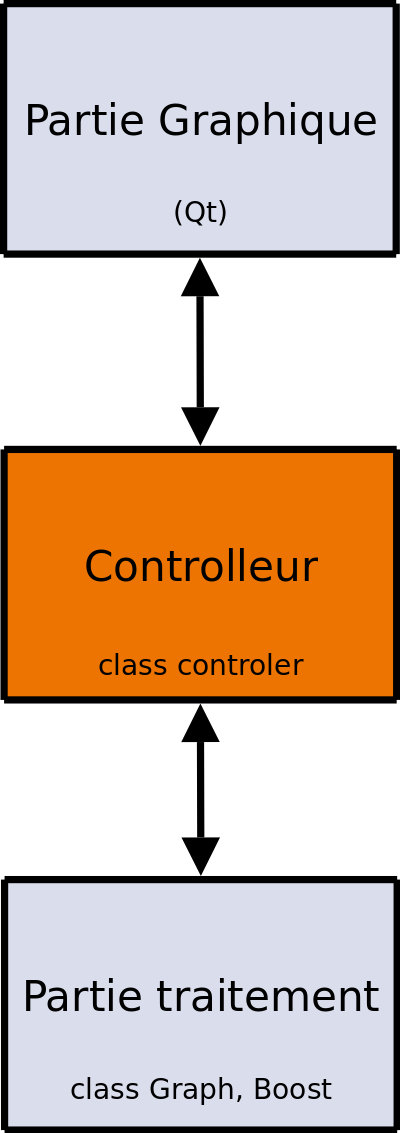
\includegraphics[height=0.3\textheight]{./schema/mvcScheme.png}
\caption{Schéma superficiel du Modèle Vue Controlleur}
\label{mvc}
\end{center}
\end{figure}

\subsubsection{La base du développement : l'objet Graph}

Dès le départ, nous savions que nous allions manipuler un graphe. Nous avons, avec l'aide de notre tuteur, créé un objet Graph à partir des classes exisantes dans \textit{Boost} nous permettant de manipuler ce graphe. En fait, cette objet est un liste d'adjacence de \textit{Boost} que nous avons spécialisé en fonction de nos besoins.

Le contenu du graphe est identifié par des descripteurs, l'un pour les sommets, \verb|vertex_descriptor| et l'autre pour les arêtes, \verb|edge_descriptor|. Bien que ces descripteurs soient des simples entiers, il ne nous était pas possible d'utiliser les numéros des AS. \textit{Boost} génère donc un entier auto-incrémenté utilisé comme identifiant vis à vis d'un objet AS contenant notamment son véritable numéro. Cette objet est stocké par le Graph.

Notre utilisation de l'objet graph ressemble à celui que l'on ferait d'une base de données. En considérant l'objet Graph comme tel, nous possèderions une table de sommets, et une table d'arêtes. La clé primaire de chacune de ces tables serait le descripteur correspondant (\verb|edge_descriptor| et \verb|vertex_descriptor|). Et nos entités seraient en faites des objets AS et ASLink (figure \ref{bdd}).

Ces objets possèdent un certain nombre d'attributs nécessaires au bon fonctionnement de boost en plus de ceux qui nous intéressent : le type et le numéro de l'AS. Pour récupérer le type de l'un de ces objets il suffit de faire \verb|graph[descriptor].type|.


\begin{figure}[H]
\begin{center}
        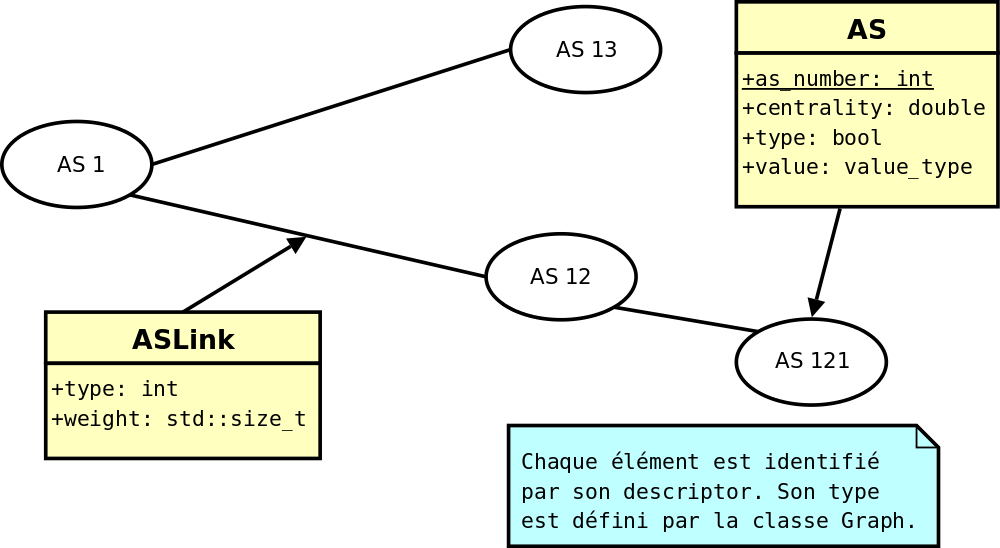
\includegraphics[width=0.8\textwidth]{./schema/bdd.png}
\caption{Représentation des types d'objet du graphe}
\label{bdd}
\end{center}
\end{figure}

\subsubsection{Représentation idéale}
Idéalement la représentation que nous souhaitions obtenir de vait tendre vers celle de la figure \ref{ideal}. 
\begin{figure}[H]
\begin{center}
        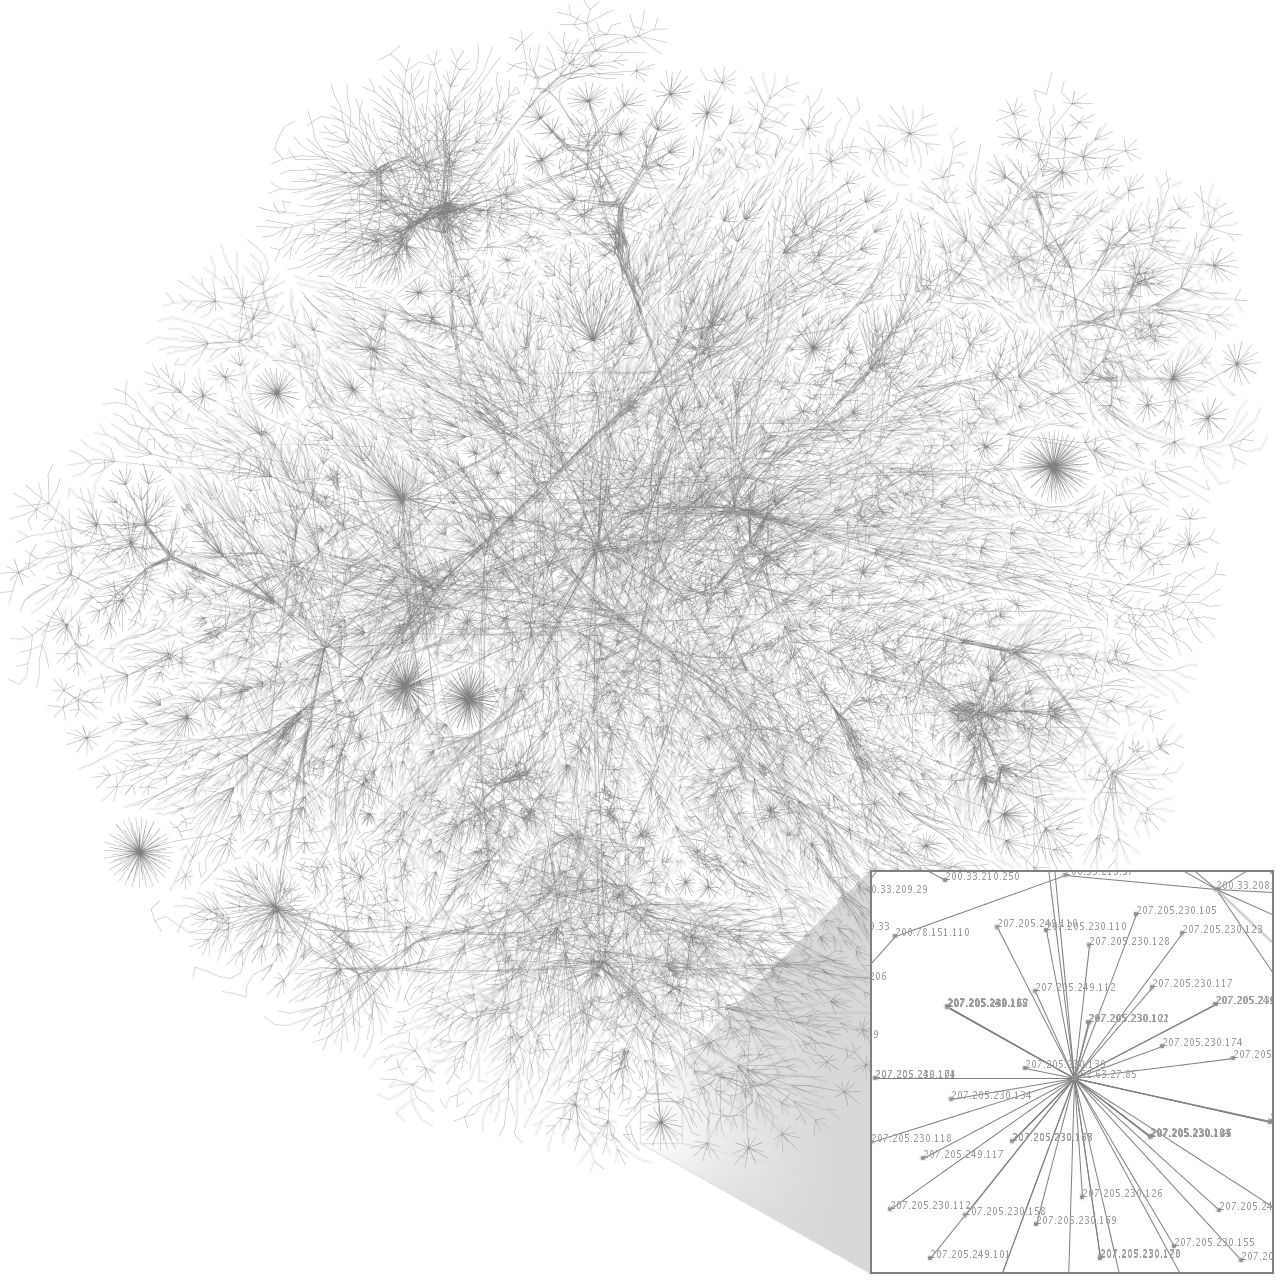
\includegraphics[width=0.8\textwidth]{./schema/Internet_map_1024_transparent.png}
\caption{Représenation idéale d'internet avec le programme}
\label{ideal}
\end{center}
\end{figure}



\pagebreak
\section{Solution r\'ealis\'ee}

\begin{frame}
 	\frametitle{Solution r\'ealis\'ee}
        \tableofcontents[currentsection,hideothersubsections]
\end{frame}

\subsection{Fonctionnalit\'es impl\'ement\'ees}
\frame
{
\frametitle{Fonctionnalit\'es impl\'ement\'ees}
\only<1>{
Fonctionnalit\'es du programme final :
\begin{itemize}
 \item R\'ecup\'eration d'informations sur un AS,
 \item Calcul du nombre de cliques maximum dans le graphe gr\^ace \`a l'algorithme de Bron and Kerbosch,
 \item Chargement d'un fichier de triplets pour \'eliminer les stubs du graphe,
 \item Zoomer sur le proche voisinage d'un AS,
 \item Revenir au graphe de base,
 \item Calculer la centralit\'e de Freeman des sommets,
 \item Filtrer les sommets selon leur centralit\'e,
 \item Filtrer les sommets selon leur num\'ero d'AS.
\end{itemize}
}
\only<2>{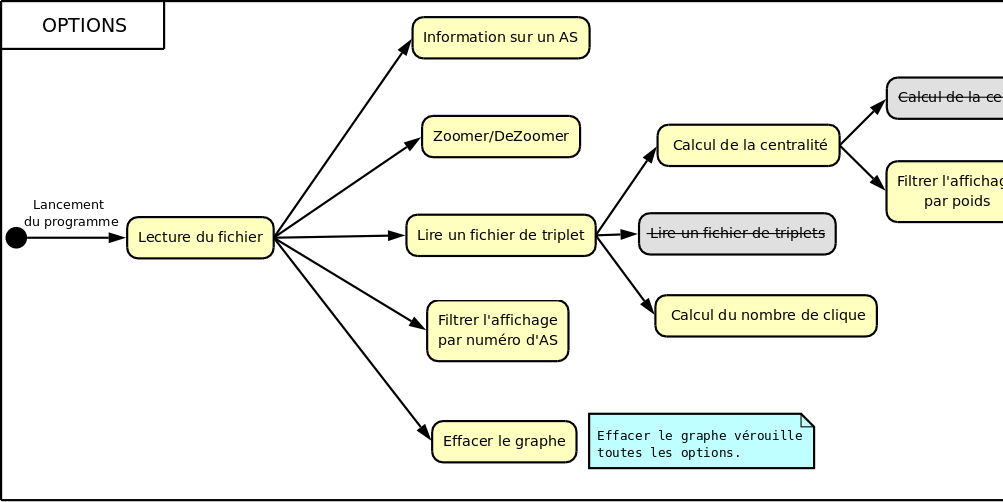
\includegraphics[width=\textwidth]{./seqMenu.png}}
}

\subsection{Rendu final}
\frame
{
\frametitle{Rendu final}
\only<1>
{
   \begin{center}
   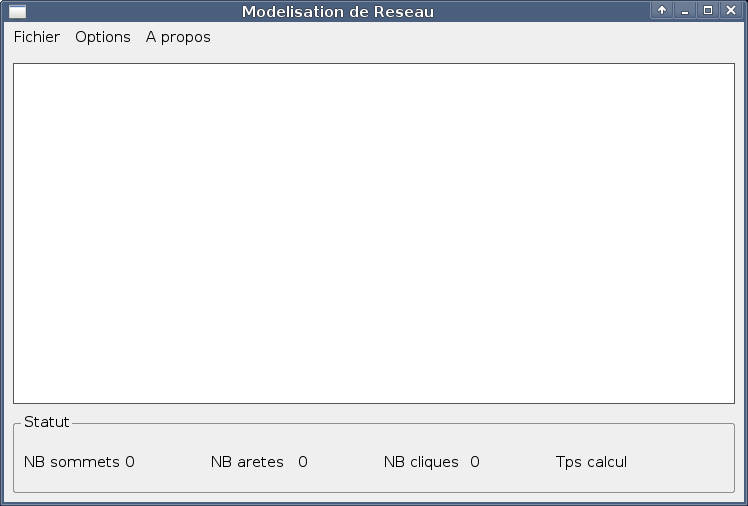
\includegraphics[width=0.9\textwidth]{ecran_programme.png}\\
   Ecran principal du programme
   \end{center}
}
\only<2>
{
   \begin{center}
   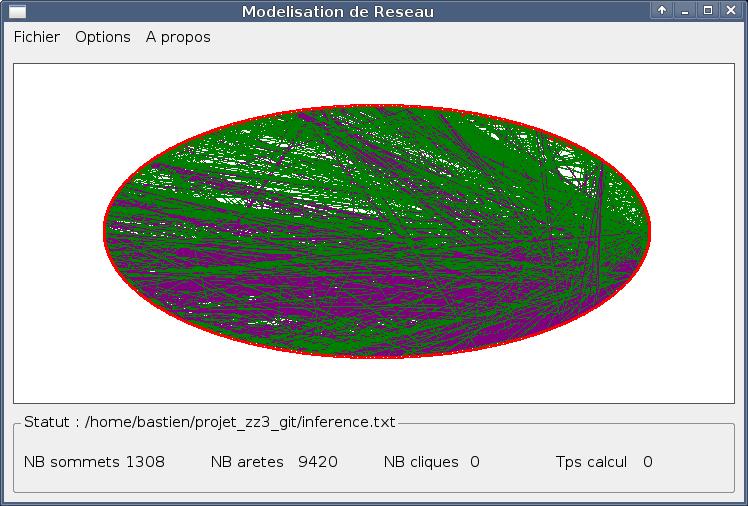
\includegraphics[width=0.9\textwidth]{ecran_graphe.png}\\
   Graphe charg\'e
   \end{center}
}
\only<3>
{
   \begin{center}
   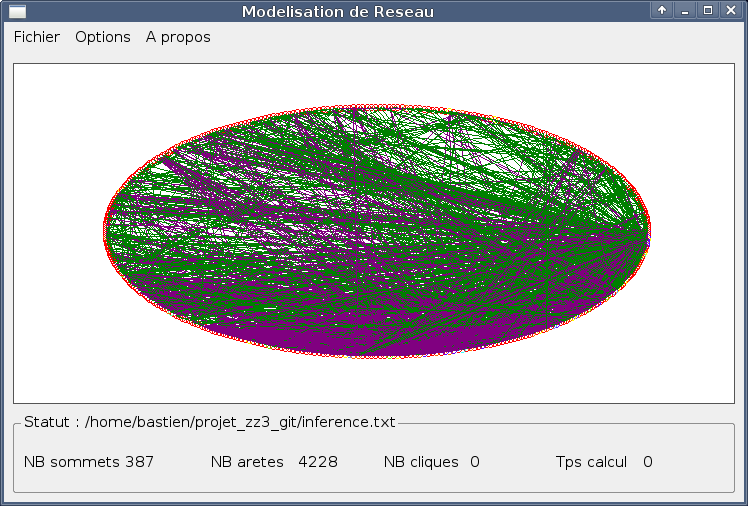
\includegraphics[width=0.9\textwidth]{ecran_graphe_nostubs.png}\\
   Stubs \'elimin\'es
   \end{center}
}
\only<4>
{
   \begin{center}
   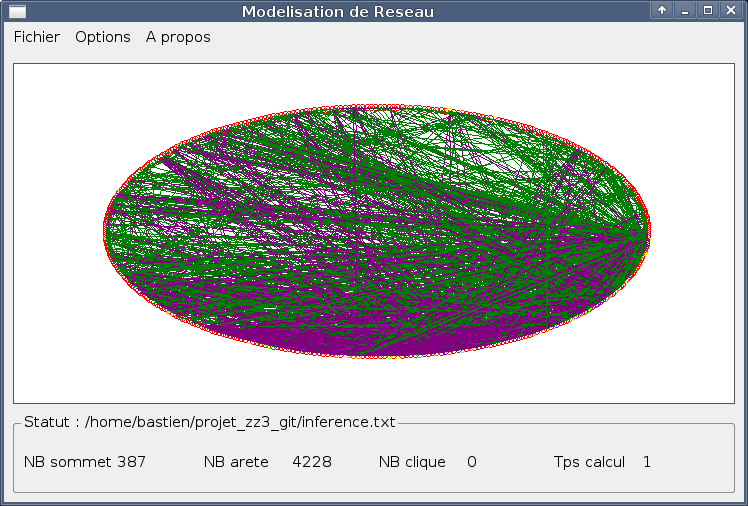
\includegraphics[width=0.9\textwidth]{ecran_graphe_centrality.png}\\
   Centralit\'e calcul\'ee
   \end{center}
}
\only<5>
{
   \begin{center}
   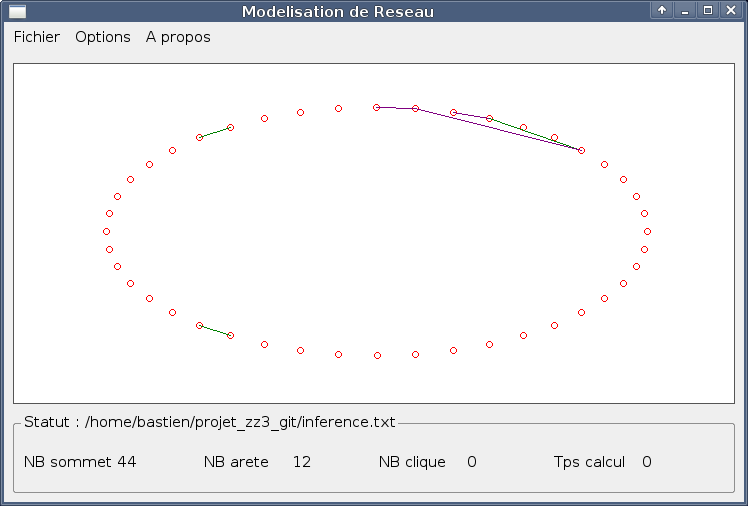
\includegraphics[width=0.9\textwidth]{ecran_graphe_filtre.png}\\
   Filtrage par num\'ero d'AS
   \end{center}
}
\only<6>
{
   \begin{center}
   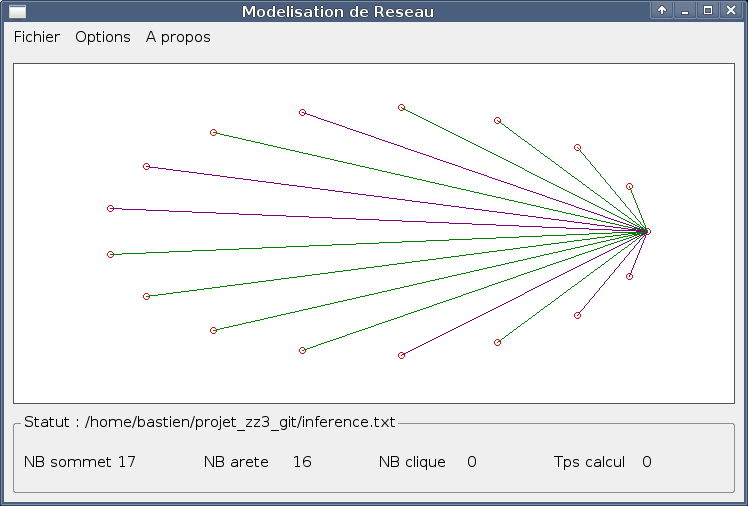
\includegraphics[width=0.9\textwidth]{ecran_graphe_zoom.png}\\
   Zoom sur un AS
   \end{center}
}
}

\pagebreak
\section{Développement du logiciel}
\subsection{Développement avec boost}
\subsubsection{Des difficultés de prise en main}
La prise en main de la librairie \textit{Boost} a été la principale difficulté du projet. En effet, la documentation fournie avec la librairie se r\'ev\`ele asses difficile \`a exploiter au premier abord. La philosophie de développement de \boost, souvent compl\`etement novatrice, est assez éloignée de ce que nous connaissions juqu'alors et finalement assez éloignée de la programmation objet (pour la partie graph) : la plupart des méthodes que nous utilisons sont en fait des fonctions. Cette librairie pousse \`a l'extr\^eme la notion de g\'en\'ericit\'e en ne proposant que des fonctions templates relatives \`a des objets conecptuels.

Pour trouver les fonctions relatives aux objets, ou comment les utiliser, il faut parcourir une dizaine de pages web de documentation par fonction expliquant comment les appeler i.e. comment créer les structures adéquates, quels arguments et structures passées en paramètres et comment les créer... Cette documentation n'est pour autant pas exhaustive et manque cruellement d'exemples, elle est clairement destinée à un public d'experts.

\subsubsection {Compilateur spécifique}
Les erreurs retournées par gcc à la compilation de la librairie sont incompréhensibles ou trop longues avec des messages d'erreur redondants et en cascade. C'est pourquoi il faut utiliser un compilateur particulier : \verb|gfilt|, utilisant perl pour analyser les erreurs de compilation et les afficher de mani\`ere intelligibles. 

Malheureusement, il n'est pas possible de compiler Qt avec ce compilateur. Nous avons donc créé un dossier de développement spécifique à \textit{Boost} que nous int\'egrions avec la partie Qt quand nous étions satisfaits du résultat. La solution la plus efficace aurait été de créer une branche sous git, mais nous n'avions pas encore décidé d'utiliser git lorsque nous avons rencontré ce problème.

\subsubsection{Bilan}

Tout au long du projet, la méthode la plus efficace pour avancer lorsque nous bloquions sur \boost a été de demander l'éclairage de notre tuteur de projet. 

\textit{Boost} est une librairie véritablement complexe dans sa construction, son code, sa compilation et son fonctionnement. L'utilisation massive des génériques et de la méta-programmation peut rendre la compilation relativement longue mais améliore grandement les performances.
~\\
Un exemple d'utilisation  concrète de la librairie \textit{Boost}, des difficultés dûes au côté ``non objet'' de la partie graphe et de ses apports en terme de performance est le traitement du fichier contenant la ``table de routage d'internet''.

\subsection{Décodeurs d'entrée}
Le fichier contenant les liens entre les AS est une succession de lignes ``\verb|AS1 AS2 TYPE|'' représentant le lien entre l'AS1 et l'AS2 et son type. Nous nous ne souhaitons conserver que le numéro de l'AS. C'est à dire une ligne de type ``\verb|1 2 TYPE|''. C'est pourquoi, la première étape lorsque nous récupérons un fichier de données est d'effectuer un traitement à l'aide de sed (figure \ref{sed}) afin de retirer les ``\verb|AS|'' et d'accélérer les traitements lors de la lecture du fichier. 
\begin{figure}[H]
   \begin{center}
      \begin{tabular}{l}
         \hline
         \verb|sed -i -e "s/AS//g" nom_du_fichier|\\
         \hline
      \end{tabular}
   \end{center}
\caption{\label{sed} Ligne de commande du traitement de sed}
\end{figure}

\subsubsection{Méthode C++}

Au début du projet, nous avons utilisé une méthode ``C++'' classique pour lire et analyser le fichier. 
Représenté en figure \ref{parse_cpp}, l'analyse dite classique est beaucoup moins performante que le celle de boost, en outre il augmente considérablement le nombre de \verb|if| imbriqués ce qui rend le code plus difficile à lire, il faut ajouter autant de \verb|else| pour la gestion des erreurs qui a été retirée du présent rapport. L'avantage de cette méthode est que nous récupérons directement \verb|asn1| et \verb|asn2| les numéros des AS correspondant à la ligne du fichier en cours de lecture en tant qu'entier.

\begin{figure}[H]
   \begin{center}
      \begin{tabular}{l}
        \hline 
        \verb|std::ifstream file(filename.c_str());|\\
	\verb|if( file.is_open() )|\\
	\verb|{|\\
   	\verb|    while(std::getline(file, line)) {|\\
      	\verb|    std::istringstream lineStream(line);|\\
      	\verb|    if(lineStream >> tempString) {|\\
        \verb|        std::istringstream in1(tempString);|\\
        \verb|        if(lineStream >> tempString) {|\\
        \verb|            std::istringstream in2(tempString);|\\
        \verb|            //Si tout rentre dans chacun des conteneurs...|\\
        \verb|            if(lineStream >> linkType && in1 >> asn1 && in2 >> asn2) {|\\
        \verb|                //TRAITEMENT|\\
        \verb|           }|\\
        \verb|        }|\\
        \verb|    }|\\
        \verb|}|\\
        \hline
      \end{tabular}
   \end{center}
\caption{\label{parse_cpp} Exemple de parsing de fichier en C++ classique}
\end{figure}




\subsubsection{Méthode Boost}
Le parsing avec boost utilise un \verb|tokenizer| et un \verb|char_separator| qui permet de décrire la chaine re\c cue en entrée. Représentée en figure \ref{parse_boost}, Cette méthode de lecture des fichiers est beaucoup plus performantes que celle du C++ classique. Si la ligne n'est pas conforme à nos critères la taille du vector de string est différente de 3 et nous retournons une erreur (ici non représentée). 

Contrairement à la version C++, si la ligne est découpée correctment, nous ne récupérons pas directement des entiers. Heureusement boost dispose d'outils de conversion entre type très performant, qui permettent notamment de ``caster'' un \verb|string| en \verb|int| (figure \ref{cast_boost}) sans pertes de performances visibles. A titre d'exemple, la méthode C++ classique prenait environ 8 secondes à s'exécuter, tandis que celle de boost ne prend plus que 4 secondes, les deux mesures contiennent les traitements et ont été exécuter sur un fichier d'environ 150000 lignes...

Au final, le traitement d'une ligne se déroule comme présenté figure \ref{file_parser}. Nous nous servons d'une map de traduction qui permet de trouver quel AS est déjà présent dans le graphe et de récupérer son \verb|vertex_descriptor|. En effet, chaque \verb|vertex_descriptor| est un entier mais il ne correspond pas au numéro de l'AS en question. Utiliser le numéro de l'AS comme \verb|vertex_descriptor| reviendrait à créer des AS fantômes, le graphe serait donc trop gros et surtout la représentation graphique et les données correspondants aux AS seraient éronnées.

Les fonctions utilisées pour ajouter des sommets et des arêtes (\verb|add_vertex| et \verb|add_edge|) au graphe montrent, encore une fois, que la partie graphe de boost est assez éloignée de l'objet.

\begin{figure}[H]
   \begin{center}
      \begin{tabular}{l}
        \hline 
 	\verb|typedef boost::tokenizer< boost::char_separator<char> > tokenizer;|\\
 	\verb|boost::char_separator<char> sep("\t");|\\
	\verb||\\
	\verb|std::ifstream file(filename.c_str());|\\
	\verb|if( file.is_open() )|\\
	\verb|{|\\
	\verb|    while(std::getline(file, line)) {|\\
	\verb|        tokenizer tokens(line, sep);|\\
	\verb|        std::vector<std::string> parts(tokens.begin(), tokens.end());|\\
	\verb|        if( parts.size() == 3)|\\
	\verb|        {|\\
	\verb|            //TRAITEMENT|\\
	\verb|        }|\\
	\verb|    }|\\
	\verb|}|\\
        \hline
      \end{tabular}
   \end{center}
\caption{\label{parse_boost} Exemple de parsing de fichier en C++ avec boost}
\end{figure}
 

\begin{figure}[H]
   \begin{center}
      \begin{tabular}{l}
        \hline 
 	\verb|asn1 = boost::lexical_cast<int>(parts.at(0));|\\
        \hline
      \end{tabular}
   \end{center}
\caption{\label{cast_boost} Exemple de ``cast'' avec les outils de boost}
\end{figure}

\begin{figure}[H]
\begin{center}
        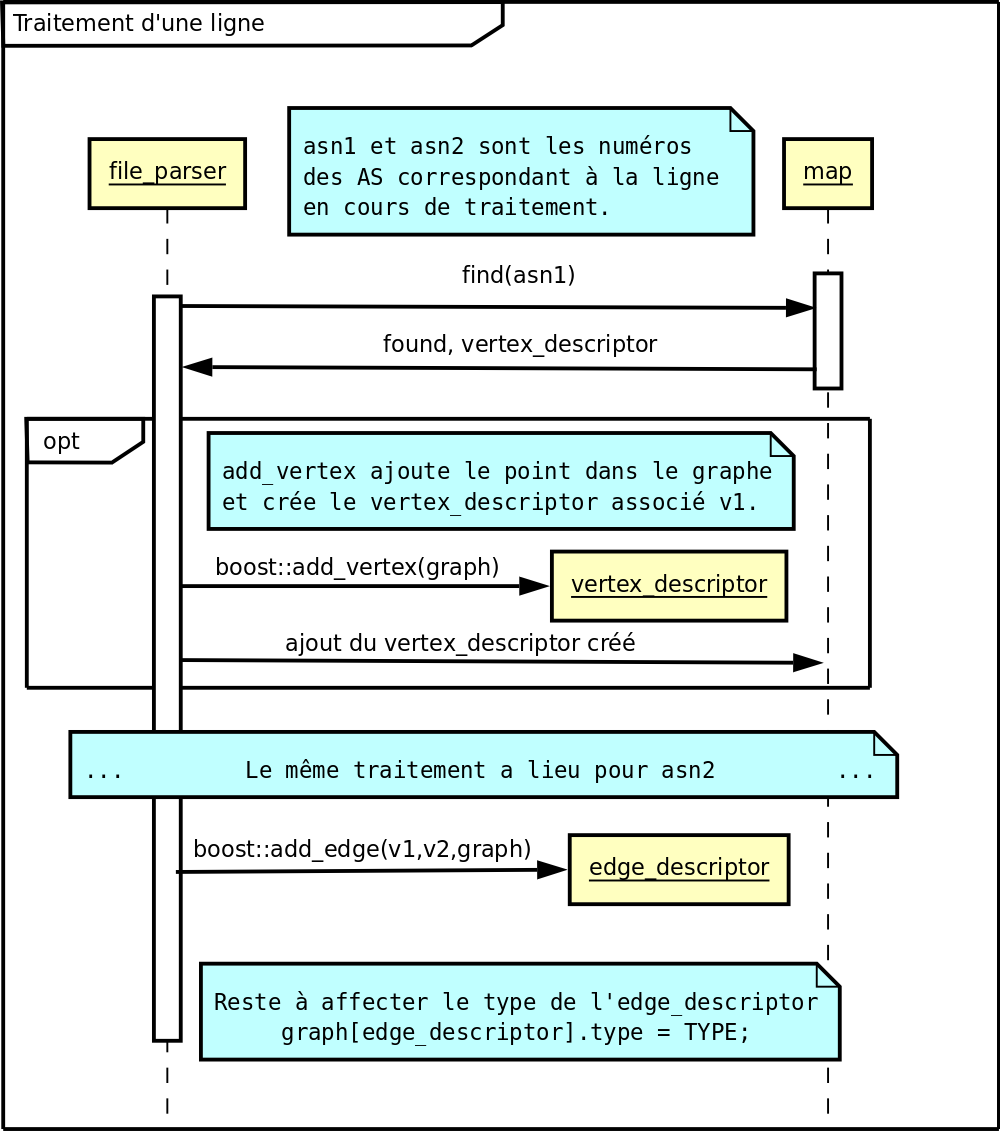
\includegraphics[width=0.7\textwidth]{./schema/file_parser2.png}
\caption{``Diagramme de séquence'' du parsing d'une ligne }
\label{file_parser}
\end{center}
\end{figure}

\subsubsection{Gestion des erreurs}

La gestion des erreurs lors du parsing du fichier se fait de manière un peu particulière. Afin de rendre le bloc parsing de fichier totalement indépendant du reste, nous avons choisi d'utiliser un simple booléen qui indique si une erreur s'est produite à cause de la lecture d'une ligne, dans le cas où l'erreur est critique (fichier inexistant, illisible ou toutes autres raisons de ce type), un autre type d'erreur est détectée. 

Pour signaler, l'erreur à la couche supérieure (le controlleur), nous remontons une exception \verb|ReaderException| de nature \verb|CRITICAL| n'importe quand ou \verb|NON_BLOCKING| une fois le graphe rempli de maniètre à empêcher ou non l'exécution de la suite du code.


\subsection{D\'eveloppement avec Qt}

\par
Le developpement avec Qt s'est fait \`a l'aide de la documentation tr\`es fournie du site de \textit{TrollTeech}. Celui propose un aper\c cu des diff\'erentes classes, ainsi qu'un certain nombre d'exemples pour aider les d\'eveloppeur.
\par
La principale difficult\'e de d\'evelopper avec Qt r\'eside dans la compr\'ehension des slots et signaux. Ce sont eux qui font toute l'interactivit\'e d'une interface graphique. Pour rendre op\'erationnelle une entr\'ee dans un menu, il faut connecter l'action qu'elle repr\'esente au slot correspondant dans son objet parent.
\par
Notre fen\^etre principale contient donc les d\'eclarations des actions correspondant aux diff\'erentes entr\'es des menus, par exemple sur la figure \ref{exemple_action_qt}, on voit la d\'eclaration de l'action permettant de quitter le programme en fermant toutes les fen\^etres.
\begin{figure}[H]
   \begin{center}
      \begin{tabular}{l}
         \hline
         \verb|QAction * _quitAct;|\\
         \hline
      \end{tabular}
   \end{center}
\caption{\label{exemple_action_qt} Exemple de d\'eclaration d'action Qt}
\end{figure}
Ensuite, lors de l'initialiation de la fen\^etre, il faut associer les 
entr\'ees du menu \`a une action, ce qui est pr\'esent\'e figure \ref{exemple_menu_qt}.

\begin{figure}[H]
   \begin{center}
      \begin{tabular}{l}
         \hline
         \verb|_fileMenu.addAction(_quitAct);|\\
         \hline
      \end{tabular}
   \end{center}
\caption{\label{exemple_menu_qt} Exemple de d'association d'action Qt \`a une entr\'e d'un menu}
\end{figure}

Enfin, il faut associer l'action \`a un slot d'un des \'el\'ement du programme si on veut que cela fasse quelque chose lorsque l'on clique sur l'entr\'e du menu. Figure \ref{exemple_initAction_qt}, on peut voir que l'action est d'abord cr\'e\'ee avec un nom, et attach\'ee \`a un objet, ici \textit{this} fait r\'ef\'erence \`a la fen\^etre principale. On assigne ensuite un raccourcis et une description \`a l'action. Finalement, l'\'etape la plus importante, on connecte l'action au slot de fermeture de la fen\^etre principale.

\begin{figure}[H]
   \begin{center}
      \begin{tabular}{l}
         \hline
         \verb|_quitAct = new QAction("Quit", this);|\\
         \verb|_quitAct->setShortcut(tr("Ctrl+Q"));|\\
         \verb|_quitAct->setStatusTip("Quit the program");|\\
         \verb|QObject::connect(_quitAct, SIGNAL(triggered()), this, SLOT(close()));|\\
         \hline
      \end{tabular}
   \end{center}
\caption{\label{exemple_initAction_qt} Exemple d'initialisation d'un action Qt}
\end{figure}

Ces \'etapes doivent \^etre r\'ealis\'ees pour toutes les actions. Il est \`a noter que l'on peut d\'eclarer \`a volont\'e des slots dans un objet. Ces slots sont en r\'ealit\'es des fonctions qui ne sont d\'eclar\'ee ni en \textit{public}, \textit{private} ou \textit{protected} mais en tant que \textit{slots} (qui peuvent \^etre publics ou priv\'es). On peut ainsi cr\'eer des fonctionalit\'es comme bon nous semble pour le programme.

\par
Lors de la cr\'eation d'un objet Qt, on utilise un macro : \verb|Q_OBJECT| qui permet la gestion des slots et signaux au moment des diff\'erentes \'etapes de la compilation.

\par
Voici l'exemple de la classe \verb|mainWindow| de notre programme qui est la fen\^etre  principale de l'interface graphique :

\begin{figure}[H]
   \begin{center}
      \begin{tabular}{l}
         \hline
         \verb|public class mainWindow : public QMainWindow|\\
\verb|{|\\
\verb|    Q_OBJECT|\\
         \verb|    protected :|\\
         \verb|        //...les attributs de la classe...|\\
         \verb|    public :|\\
         \verb|        //...les méthodes publiques de la classe...|\\
         \verb|    public slots :|\\
         \verb|        //...les slots publiques de la classe...|\\
\verb|}|\\
         \hline
      \end{tabular}
   \end{center}
\caption{\label{exemple_mainWindow_qt} Exemple d'un classe Qt}
\end{figure}

La classe mainWindow h\'erite de la classe QMainWindow de Qt qui est la classe pour les fen\^etres principales d'un programme dans laquelle, on ajoute tous les \'el\'ements composant le programme (menu, zone de dessin, barre de statut) sous forme d'attributs de classe.
Un certains nombre de m\'ethodes publiques sont d\'efinies pour int\'eragir avec ces \'el\'ements, par exemple : changer tel ou tel affichage dans la zone de dessin.
Enfin, un certain nombre de slots publiques correspondent aux actions r\'ealisables dans les menus. Ces slots sont des fonctions qui sont appel\'ees en r\'eponse \`a un clique de souris sur un menu ou un bouton.

\subsection{Expérimentation sur le code}
Notre connaissance grandissante des librairies utilisées nous a permis de pratiquer diverses expérimentations sur nos algorithmes, traitements et affichages.
\subsubsection{Expérimentation avec Qt}
\paragraph{}
Au cours de la premi\`ere phase du projet, nous avions un module de lecture sur fichier vraiment lent, aussi, il arrivait souvent lors du chargement du fichier que notre fen\^etre principale devienne grise. En fait, l'OS cherchait \`a signifier par l\`a que la fen\^etre ne réponde plus depuis un moment, ce qui \'est normal au vu des traitements réalisés par le programme.

Aussi nous avons décidé d'afficher une petite fen\^etre annon\c cant ``un calcul est en cours''. Pour cela, nous avons effectué des recherches sur les \textit{QThread}. Ceux-ci devaient permettre \`a notre fen\^etre de chargement de continuer d'\^etre active m\^eme si la fen\^etre principale cessait de répondre.

Nos recherches nous ont appris que Qt ne permet pas de gérer l'affichage en dehors du thread principal. Donc, une fen\^etre de chargement doit être g\'er\'ee par le m\^eme thread que la fen\^etre principale. Ce sont les calculs qui doivent \^etre effectu\'es par un autre thread.

Avec l'arriv\'ee du second module de lecture de fichier, le processus est devenu plus rapide et l'utilit\'e de cette fen\^etre pour faire patienter l'utilisateur nous semble moins importante, aussi l'id\'ee a été rel\'egu\'ee au second plan, et finalement ne se retrouve pas impl\'ement\'ee dans le programme final.

\subsubsection{Expérimentation avec boost}

\paragraph{Kamada Kawai Layout}
Kamda Kawai Layout est une fonctions de \boost permettant de calculer les coordonn\'ees des points d'un graphe. Contrairement \`a Circle Graph Layout qui les pla\c ce sur un cercle, Kamada kawai les organise selon leur poids.
La fonction Kamada Kawai n'est pas impl\'ement\'ee dans la version finale.

\paragraph{Recherche des peers\\}
\par La recherche des peers a été développé en deux étapes. La première étape fut de trouver un moyen de recenser les Peers à partir de fichier de routage uniquement, afin de permettre de trouver les cliques avec un algorithme ``maison''. Cette méthode se basait sur le ciblage des AS qui n'avaient ni client, ni peer : ce sont n\'ecessairement des stubs. A ce moment là, nous stockions plusieurs graphs dans l'objet contrôleur dont le principale et celui sans les stubs.

Cette méthode présupposait que le fichier était ordonné et bien que ce soit le cas avec le fichier qui nous servait de base cela ne le serait pas forcément avec tous les fichiers devant être utilisés. Et ordonner manuellement un fichier de 100000 lignes reléverait d'un exploit digne d'un héros de la mythologie grecque. Ordonner ce fichier avec une fonction dédiée était possible, mais il fallait trouver un moyen plus ``propre'' et performant.

\par Notre tuteur de projet, Monsieur Meulle, nous a fourni un nouveau fichier, avec des relations entre AS sous la forme de triplets, permettant d'identifier tr\`es rapidement les AS feuilles.
Les liens entre AS sont plac\'ees sous la forme : {AS1, AS2, AS3} signifiant que pour joindre l'AS3, l'AS1 a dû passer par l'AS2. Les AS du milieu sont donc forcément des AS de transit, les AS stubs sont alors facilement identifiables comme \'etant tous les autres... 

C'est à ce moment-là que le structure actuelle du programme a été clairement établie, nous ne stockons qu'un seul graphe dans le controlleur et celui-ci réalise un traitement de création d'un graphe spécifique en fonction de ce qui lui ait demandé. Un fonctionnement proche d'une base de données décrit en \ref{mvcText}. 

En outre, l'utilisation du modèle MVC nous a permis de continuer à travailler sur l'ensemble du projet. Pendant que l'un d'entre nous apportait les corrections nécessaires à la partie lecture de fichier, l'autre continuait de développer l'interface graphique. La fusion des deux parties s'est révélée triviale le contrôleur ne perdant pas de fonctionnalités, il ne restait plus qu'à l'adapter et à lui en ajouter de nouvelles.


\end{document}
